\documentclass[a4paper,10pt]{article}
\usepackage[utf8]{inputenc}
\usepackage{amsmath,amsfonts,amssymb,amsthm,epsfig,epstopdf,array}
\usepackage{tikz}
\usepackage{caption}
\usepackage{pgfplots}
\usepackage{ulem}
\usepackage{pifont}% http://ctan.org/pkg/pifont
\usepackage{hyperref}
\begin{document}
\subsection{Limiting Amplitude and Limiting Absorption Principle}
In this section we perform several numerical experiments,
with the normalization chosen as $\epsilon_0=\mu_0=1$, $\omega=c=1$. 
Also, we set $m_e=1$ and $e=-1$. From this it follows that $w_c=-B_0$ and $w_p^2=N_e$. 
We consider the following two cases:
\begin{itemize}
 \item case $N_e\neq \operatorname{const}$, no resonance
 \item case $N_e\neq \operatorname{const}$, resonance
\end{itemize}
For every fixed absorption rate $\nu$, in the time domain we choose the boundary conditions of the form
\begin{align}
\label{eq:bcs}
\left.\partial_t H\right|_{x=-L}&=-\left.\partial_x E_y\right|_{x=-L}=G\sin(t),\; G\in \mathbb{R}, \\
 \nonumber
 \left.\partial_t H\right|_{x=H}&=0,
\end{align}
and zero initial conditions, and in the frequency domain
\begin{align*}
 \left.\partial_x \hat{E}_y\right|_{x=-L}&=G,\\
 \left.\partial_x \hat{E}_y\right|_{x=H}&=0.
\end{align*}
We compute the solution $\mathbf{E}^{\nu}(t)$ for large $t$ in the time domain (the solution computed numerically at the time step $n$ is denoted by $\mathbf{E}^{\nu}_{n}$), and the solution $\hat{\mathbf{E}}^{\nu}$ in the frequency domain. 
Our goal is to check whether
\begin{align*}
\lim_{t\rightarrow+\infty}\mathbf{E}^{\nu}(t)=\Im\left(\hat{\mathbf{E}}^{\nu}\exp(it)\right).
\end{align*}

\subsubsection{No-Resonance Case}
We choose the parameters so that in the frequency domain, for the limiting amplitude problem, $\hat{E}_{2}$ satisfies 
the Airy equation (\ref{}). 

We set $\omega_c=0$ (thus $\delta(x)=0$), $\omega=1$ (hence $\alpha(x)=1-N_e(x)$), 
choose the domain as $[-0.5, 10]$ and set the electron density $N_e(x)=1+x$. Importantly, $N_e(x)>0$ on the whole interval.
The boundary conditions in (\ref{eq:bcs}) are chosen as $G=Ai'(0.5)$. 
In all the experiments in this section the CFL number was chosen to be equal to 0.5.


First let us fix $\nu=1e-2$. 
To demonstrate that the limiting amplitude principle indeed holds, we fix a point $x=x_c$ 
inside the domain $(-L,\; H)$ and plot the dependence of the solution $E_{2}^{\nu}(x_c,t), \; \hat{E}_2^{\nu}(x_c)\mathrm{e}^{it}$ 
on time $t$ for a range of $t\gg 1$ in Figure \ref{fig:nu1e2_harmon}.  

\begin{figure}[htb]
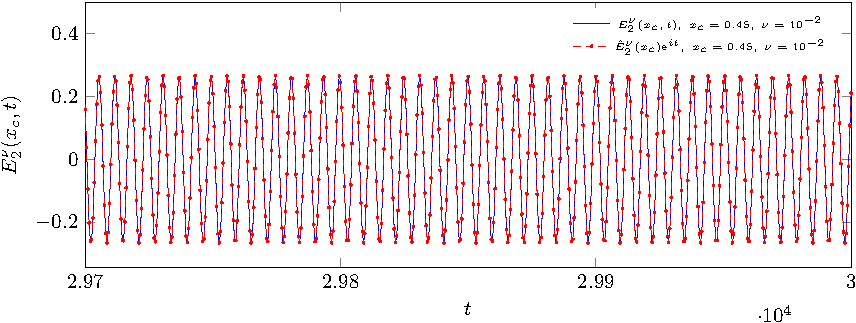
\includegraphics[width=0.9\textwidth]{figure_nu1e2-crop.pdf}
 \label{fig:nu1e2_harmon}
\end{figure}

In Figure \ref{fig:nu1e2_harmon2} (left figure) we compare this solution to the computed $\hat{E}_2^{\nu}\mathrm{e}^{it}$, for
fixed values of $t$. Both solutions appear to be in close agreement. 
\begin{figure}[htb]
 \begin{tabular}{ll}
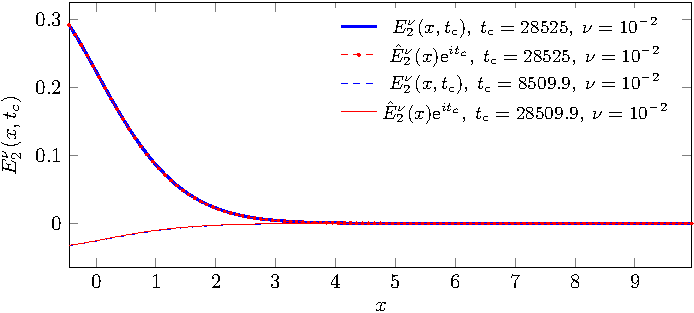
\includegraphics[width=0.5\textwidth]{figure_nu1e2_2-crop.pdf}
&
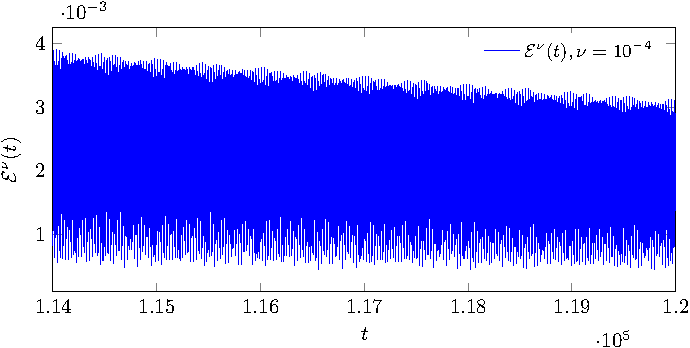
\includegraphics[width=0.5\textwidth]{figure_error_nu1e4-crop.pdf}\\
\end{tabular}
\caption{In the left figure we show the solution to (\ref{}) for $\nu=10^{-2}$, for two fixed moment of times. In the right figure 
the dependence of the error (\ref{eq:error}) on time for $\nu=10^{-4}$ is demonstrated. 
We can see that the error is decreasing.}
 \label{fig:nu1e2_harmon2}
\end{figure}
The computed $L_2$ error
\begin{align}
\label{eq:error}
\mathcal{E}(t)=\|\Im\left(\hat{E}_y^{\nu}\exp(it)\right)-E_y^{\nu}(t)\|_{L_{2}(-L;H)}.
\end{align}
for $\nu=1e-2$ did not exceed $1.1e-3$ for values of $t\in \left(28501,  30000\right)$. 

Figure show the solutions at fixed time steps for $\nu=1e-4$. As before, 
to demonstrate that the limiting amplitude principle indeed holds, we fix a point $x=x_c$ 
inside the domain $(-L,\; H)$ and plot 
the dependence of the solution $E_{2}^{\nu}(x_c,t)$ on time $t$ for a range of $t\gg 1$. 
The error (\ref{eq:error}) for $\nu=1e-4$ at the time interval $[228000.05,\; 240000.05]$ does not exceed 2.8e-4. 
One of our observations was that for smaller $\nu$ one requires more time steps to achieve the limiting amplitude solution, 
c.f. e.g. Figure \ref{fig:nu1e2_harmon2}. 
We were not able to obtain the limiting amplitude solution for $t<3\cdot 10^{4}$, unlike in the case of $\nu=10^{-2}$. 
For example, for $\nu=1e-6$ we were not able to reach the limiting amplitude solution even on the time interval $t\leq 1.92e6$, 
see Figure \ref{fig:nu1e4_harmon}. 
\begin{figure}
\begin{tabular}{c}
 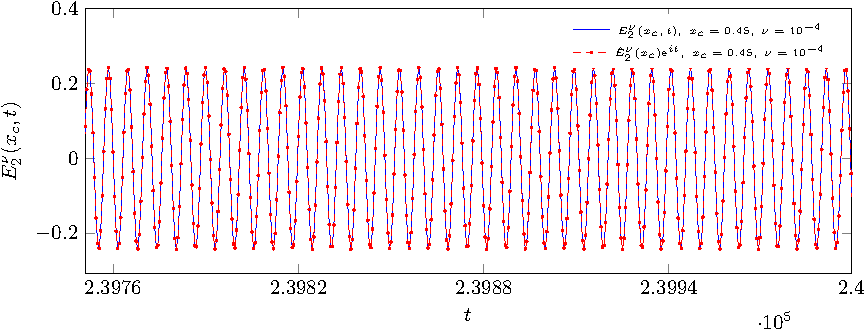
\includegraphics[width=\textwidth]{figure_nu1e4-crop.pdf}\\
 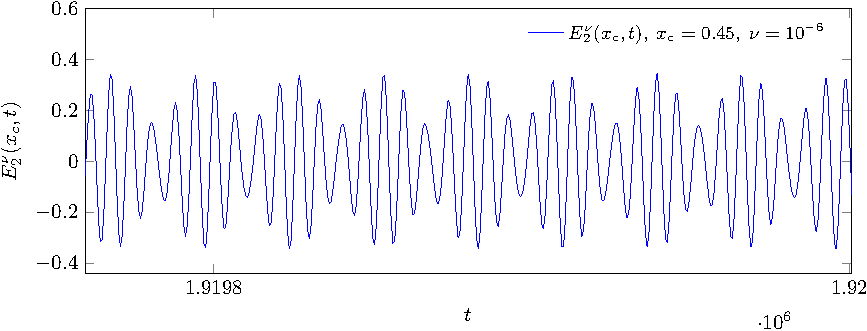
\includegraphics[width=\textwidth]{figure_nu1e6-crop.pdf}\\
\end{tabular}
\caption{In the upper figure we plot the dependence of the solution $E_{2}^{\nu}(x_c,t)$ on time $t$, with $\nu=10^{-4}$ and $x_c=0.45$. 
In the lower figure we show the solution for $\nu=10^{-6}$ at the same point $x_c$, for larger times. As we can see, for 
$\nu=10^{-4}$ the limiting amplitude solution was reached for large $t$. For $\nu=10^{-6}$ we were not able 
to obtain the limiting amplitude solution even for $t\approx 1.9e6$. }
  \label{fig:nu1e4_harmon}
\end{figure}

\subsubsection{Resonance Case}
For the resonance case, we choose the parameters as given in Table \ref{}.
\begin{tabular}{cc}
$L$ & 5\\
$H$ & 19\\
$\omega_c$ &  $\sqrt{0.5}$\\
$N_e(x)$ &  $\left\{
 \begin{array}{cc}
  0.25, & x<-0.5,\\
  \frac{1+x}{2}, & x\geq -0.5, x\leq 9\\
  5, & x>9.
 \end{array}\right.$
 $G$ as in (\ref{eq:bcs}) & 0.11 \\
\end{tabular}
Since $\alpha(x)=(1-2N_e(x))$, $\alpha(0)=0$. Clearly, $\delta(0)\neq 0$ (resonance case).





The electron density 
\begin{align*}
 N_e(x)=
 \left\{
 \begin{array}{cc}
  0.25, & x<-0.5,\\
  \frac{1+x}{2}, & x\geq -0.5, x\leq 9\\
  5, & x>9.
 \end{array}\right.
\end{align*}

Since $\alpha(x)=(1-2N_e(x))$, $\alpha(0)=0$. Clearly, $\delta(0)\neq 0$ (resonance case).

We solve this problem on the interval $[-5,\; 19]$.
The boundary condition is
\begin{align*}
 \partial_y E(-5)=-\partial_t H(-5)=-0.11\cos(t).
\end{align*}



We choose $\omega_c:=\sqrt{0.5}$ and $\omega=1$.


In all the experiments we choose in the time domain $\Delta x=0.0125$ and CFL=0.9.



The electron density 
\begin{align*}
 N_e(x)=
 \left\{
 \begin{array}{cc}
  0.25, & x<-0.5,\\
  \frac{1+x}{2}, & x\geq -0.5, x\leq 9\\
  5, & x>9.
 \end{array}\right.
\end{align*}



We solve this problem on the interval $[-5,\; 19]$.
The boundary condition is
\begin{align*}
 \partial_y E(-5)=-\partial_t H(-5)=-0.11\cos(t).
\end{align*}


The results for $\nu=1e-2$ (chosen as a parameter both in frequency and time domain) 
are shown in Figure \ref{resonance_nu1e2}. 



\end{document}